\chapter{Introducción Específica} % Main chapter title

\label{Chapter2}

%----------------------------------------------------------------------------------------
En este capítulo se presenta una visión general del equipo desarrollado y se muestran algunos aspectos de la planificación del proyecto.


\section{Esquema general del sistema}

El producto básicamente debe permitir controlar una carga eléctrica a través de comandos que se le envían desde un teléfono móvil. Un esquema básico del sistema puede verse en la Figura \ref{fig:esquema_sistema}. Dentro del contexto de este trabajo final, se desarrolló un prototipo funcional del equipo. Por lo tanto, es un producto que cumple todas la funciones que va a tener el equipo final, pero que no busca cumplir con características mecánicas y estéticas que si van a estar presentes en el producto comercial. Una descripción detallada del hardware desarrollado se encuentra en la Sección \ref{section:hardware}.

\begin{figure}[h]
	\centering
	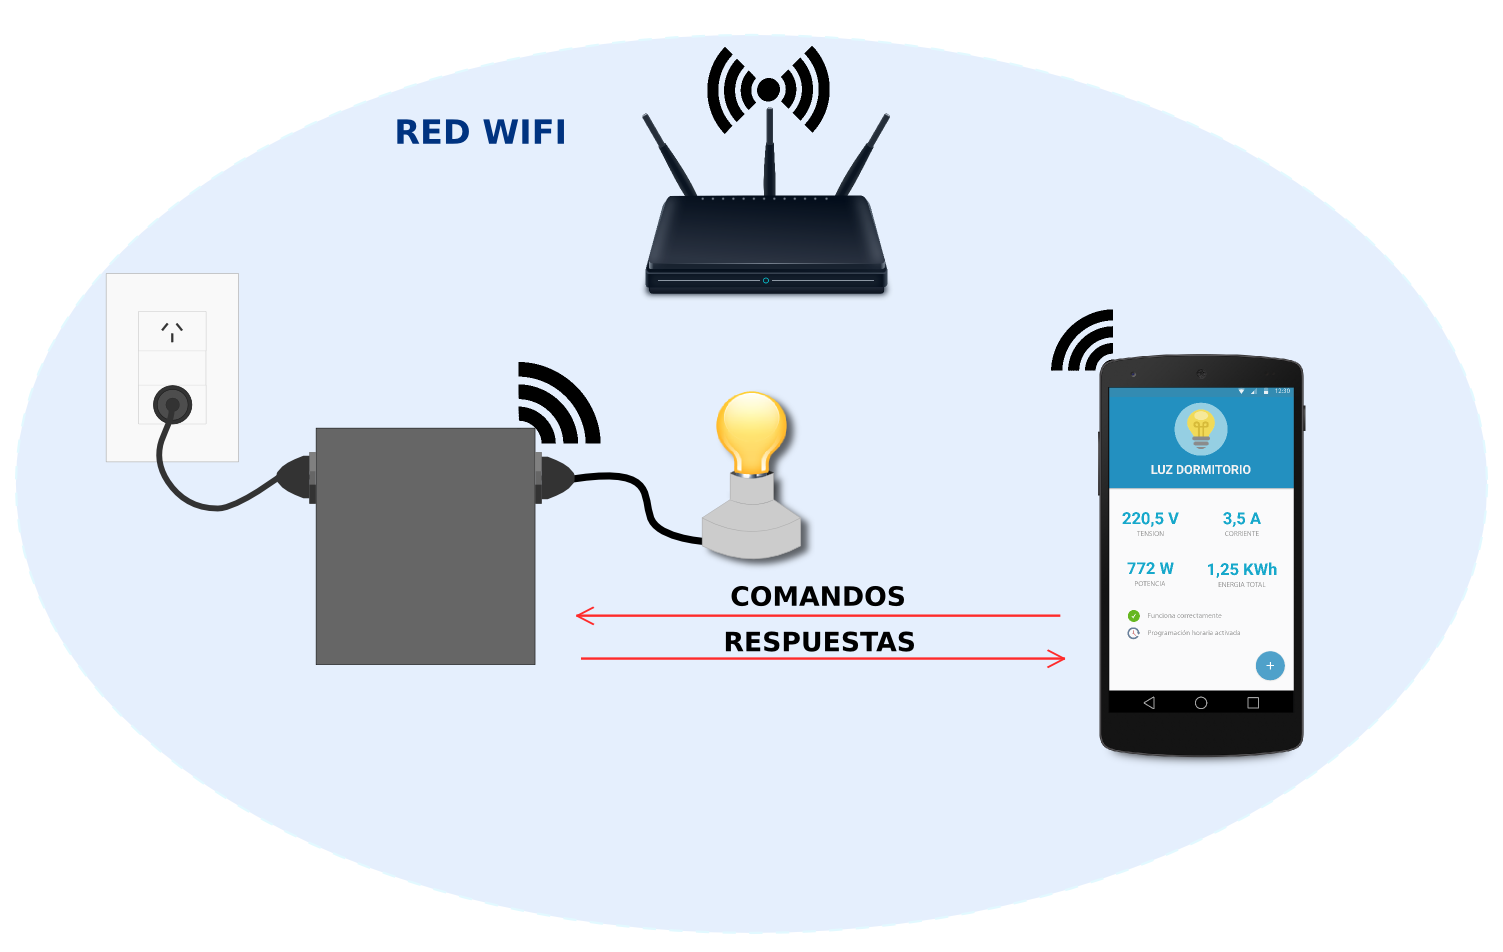
\includegraphics[width=12cm]{./Figures/2_1_esquema_sistema.png}
	\caption{Esquema general del sistema propuesto en este proyecto, compuesto por un Smart Plug y la aplicación móvil.}
	\label{fig:esquema_sistema}
\end{figure}

Cuando se adquiere un Smart Plug, lo primero que debe hacerse es incorporarlo a la red WiFi del hogar. Se eligió que la comunicación fuera a través de esta red, ya que con el paso de los años cada vez es más común que en las casas esté disponible este servicio, debido a que muchos otros dispositivos electrónicos necesitan de una conexión a Internet.

Para agregar el Smart Plug a la red, se puede proceder de dos formas: WPS o configurando la red en el Smart Plug. En el primer caso, el proceso es sumamente sencillo: simplemente se debe presionar el pulsador que se encuentra en la placa del Smart Plug (el led verde comenzará a destellar) y luego presionar el pulsador de WPS que se encuentra en el router WiFi. Una vez hecho esto, el Smart Plug se incorpora a la red. 

Sin embargo, muchos routers hogareños no cuentan con la funcionalidad de WPS, por lo que existe otra forma de configurar la red WiFi. Esta consiste en establecer al Smart Plug como un punto de acceso temporario. Para esto se debe mantener presionado el pulsador en la placa del Smart Plug durante 5 segundos. Cuando el led verde comienza a destellar, indica que el punto de acceso fue creado. Luego de esto se debe conectar un dispositivo móvil a la red WiFi creada por el Smart Plug. Una vez conectado, mediante un \textit{browser} se debe entrar a la página de configuración de la red WiFi (\textit{http://config}) y cargar los parámetros de la red a la que se desea conectar el Smart Plug: SSID de la red, tipo de seguridad y clave.

Cuando el Smart Plug se encuentra conectado a la red WiFi ya puede comenzar a ser comandado mediante la aplicación móvil. El único requerimiento para que el sistema funcione es que tanto los Smart Plugs como el teléfono en el que está la aplicación se encuentren en la misma red WiFi. En el alcance de este trabajo no estaba contemplado el desarrollo de la infraestructura para poder comandar los Plugs desde fuera del hogar.

La aplicación lista todos los Plugs que encuentra en la red WiFi y permite: encender/apagar la carga, conocer algunos parámetros eléctricos (tensión corriente, potencia y energía), configurar horarios de encendido y apagado, visualizar mediciones históricas de potencia y energía. La cantidad de Smart Plugs que puede gestionar la aplicación no está limitada, por lo que se pueden controlar numerosos dispositivos eléctricos dentro de una casa.

Además de poder enviar comandos a los Smart Plugs cuando el usuario lo requiere, la aplicación inicia un servicio en Android que se encarga de realizar consultas periódicamente a todos los Smart Plugs que tiene registrados, aun cuando la aplicación se encuentre cerrada. Mediante estas consultas, la aplicación va a poder conocer: si la carga está encendida o no, las últimas mediciones, los cambios en las configuraciones del equipo, etc. De esta forma se logra que una aplicación móvil puedan comandar y configurar un Smart Plug y todas las demás que tengan registrado a ese mismo Plug se mantengan actualizadas con estos cambios. Una explicación más detallada del funcionamiento y del diseño de la aplicación móvil se encuentra en la Sección \ref{section:app}.

Finalmente, la comunicación entre los Smart Plugs y la aplicación móvil se basa en conexiones TCP iniciadas por la aplicación. Sobre TCP se desarrolló un protocolo propio que permite enviar comandos a los Plugs tanto para que realicen acciones como para leer/escribir valores de ciertos registros también definidos por el protocolo diseñado. Este protocolo es explicado en mayor profundidad en la Subsección \ref{subsection:protocolo}.



\begin{figure}[!h]
	\centering
	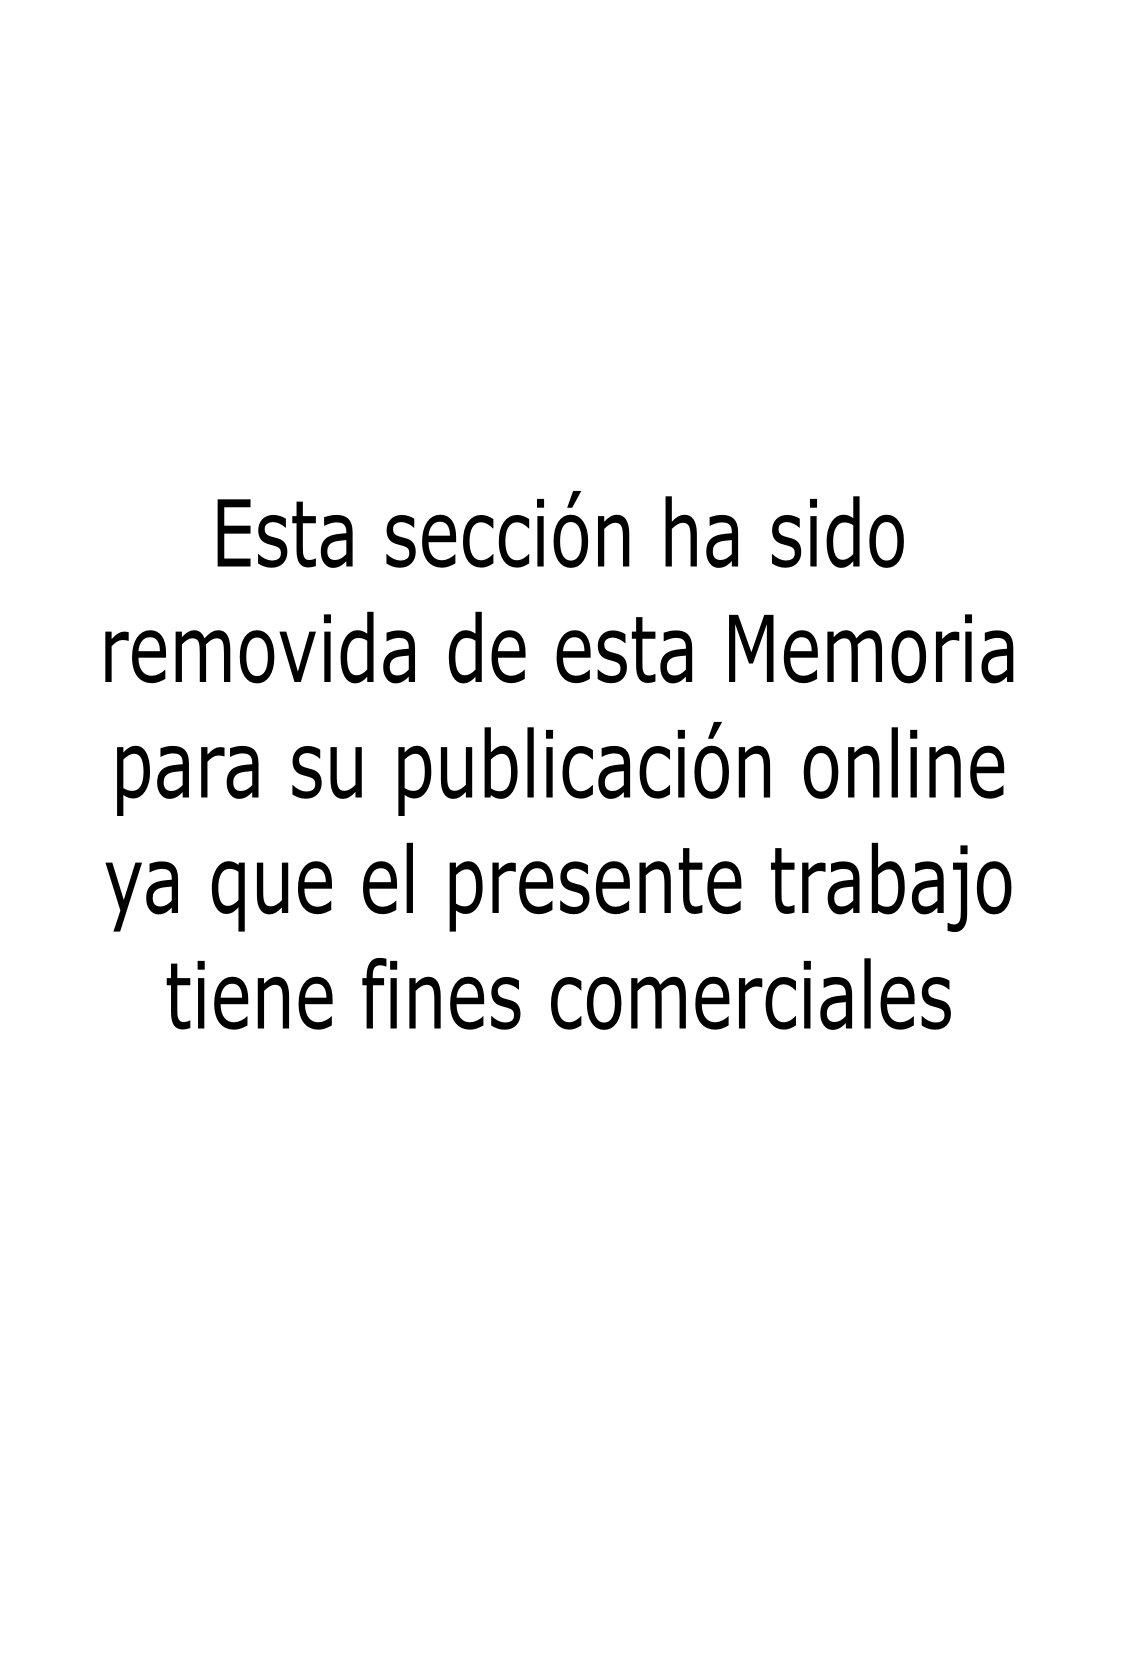
\includegraphics[width=14cm]{./Figures/comercial.png}
\end{figure}



\begin{figure}[!h]
	\centering
	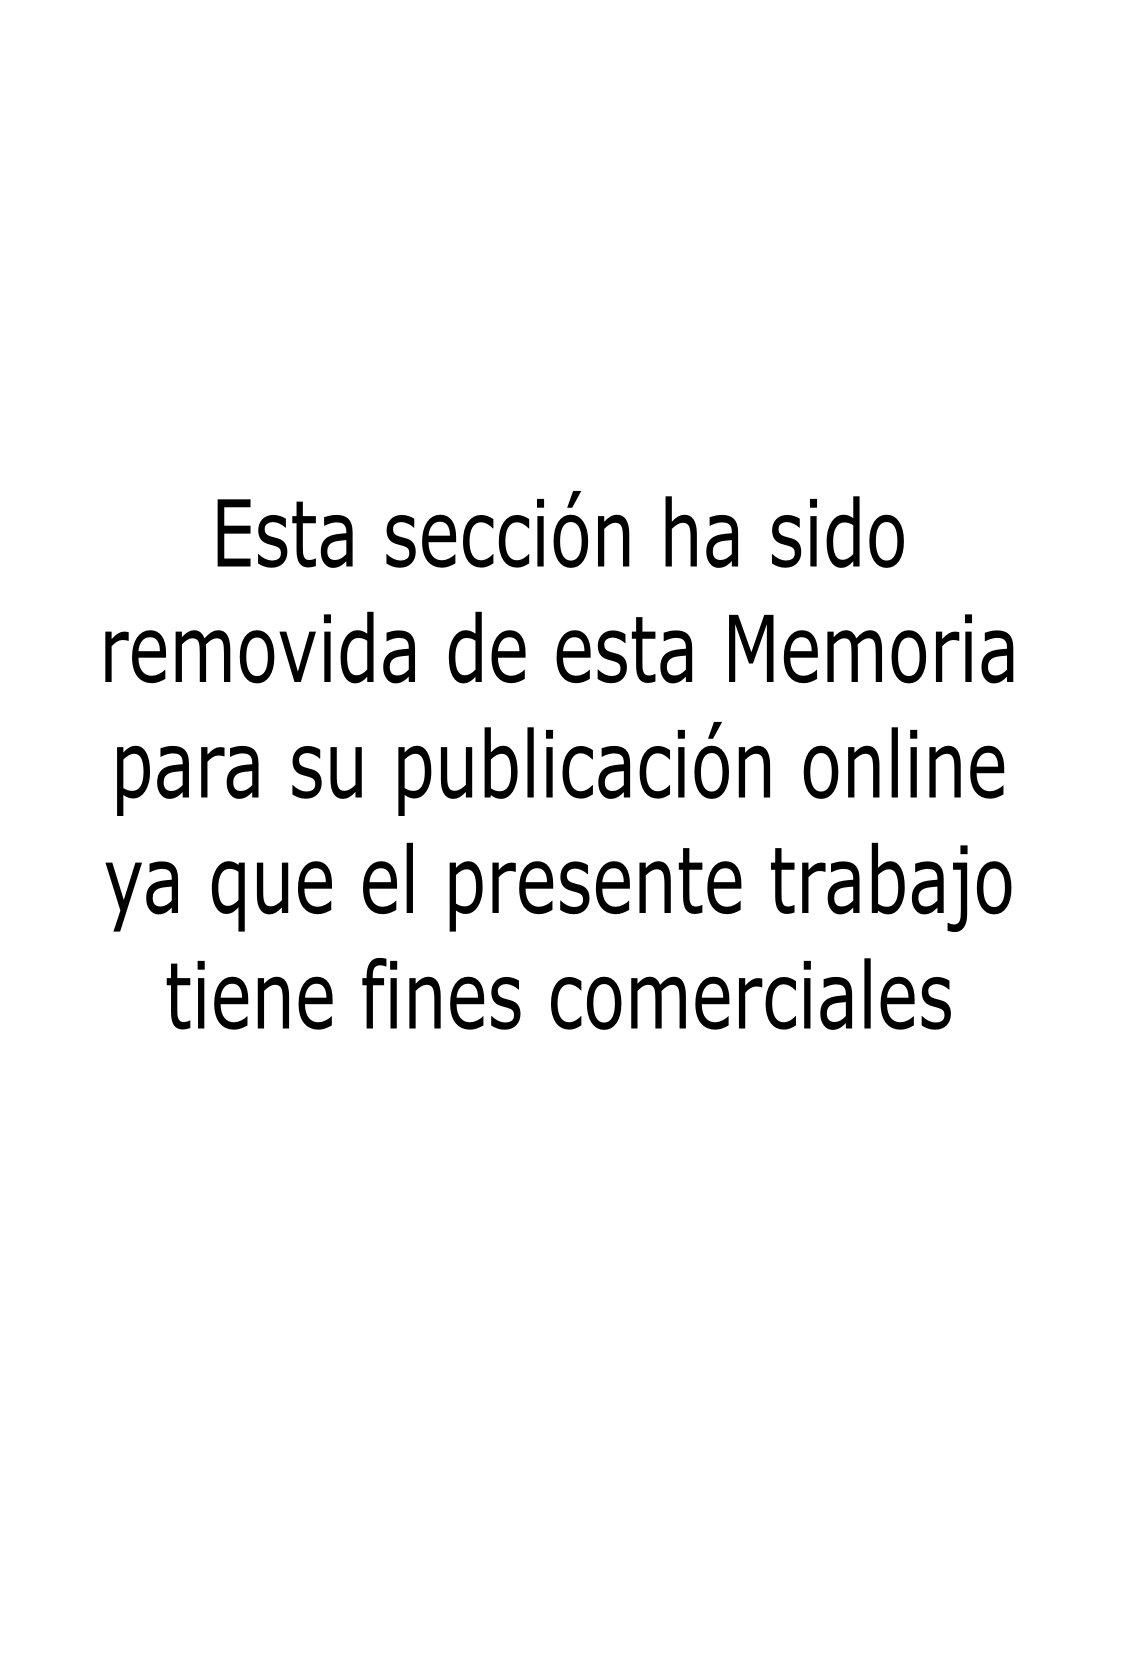
\includegraphics[width=14cm]{./Figures/comercial.png}
\end{figure}
